\documentclass[border=4pt]{standalone}
% Preámbulo común de las figuras. Cada figura es un documento standalone
% que se compila a SVG con scripts/build_figures.sh
\usepackage[utf8]{inputenc}
\usepackage{amsmath}
\usepackage{tikz}
\usepackage[american, siunitx]{circuitikz}
\usetikzlibrary{arrows.meta,calc,decorations.pathmorphing,patterns}
\tikzset{
  >={Stealth[length=2.2mm]},
  eje/.style={->, thin},
  hilo/.style={thick},
}
% Paleta común: tonos medios legibles sobre fondo claro
\definecolor{azul}{RGB}{31,94,168}
\definecolor{rojo}{RGB}{192,57,43}
\definecolor{verde}{RGB}{39,128,73}
\definecolor{naranja}{RGB}{211,120,30}
\definecolor{morado}{RGB}{125,60,152}

\begin{document}
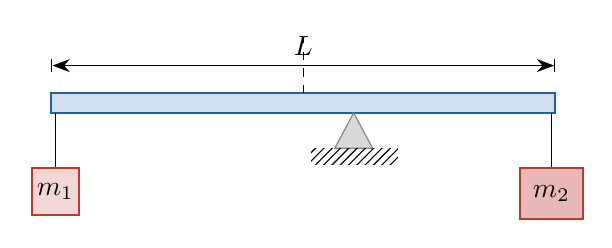
\begin{tikzpicture}[scale=1.0]
  \filldraw[draw=azul, fill=azul!20, thick] (0,1.0) rectangle (6.4,1.25);
  \filldraw[draw=gray, fill=gray!30] (3.84,1.0) -- (3.6,0.55) -- (4.08,0.55) -- cycle;
  \fill[pattern=north east lines] (3.3,0.35) rectangle (4.4,0.55);
  \draw[thin] (0.05,1.0) -- (0.05,0.3);
  \draw[thin] (6.35,1.0) -- (6.35,0.3);
  \filldraw[draw=rojo, fill=rojo!20, thick] (-0.25,-0.3) rectangle (0.35,0.3);
  \filldraw[draw=rojo, fill=rojo!35, thick] (5.95,-0.35) rectangle (6.75,0.3);
  \node at (0.05,0) {$m_1$};
  \node at (6.35,-0.02) {$m_2$};
  \draw[|<->|] (0,1.6) -- node[above]{$L$} (6.4,1.6);
  \draw[dashed] (3.2,1.25) -- (3.2,1.95);
\end{tikzpicture}
\end{document}
